\documentclass[18pt]{beamer}
%% SLIDE FORMAT
\usetheme{Boadilla}
\usepackage[utf8]{inputenc}
\usepackage{algpseudocode}
\usepackage{multicol}

\title[Programmieren Tutorium]{8. Programmieren Tutorium:\texorpdfstring{\\}{} Exceptions}
%\subtitle{Fancy Stuff}
\author{Konstantin Zangerle \texorpdfstring{\\}{} info@konstantinzangerle.de}
\date{21. Dez 2015}

\usepackage{listings}
\usepackage{xcolor}

\setlength\columnseprule{.4pt}

\definecolor{mygreen}{rgb}{0,0.6,0}
\definecolor{mygray}{rgb}{0.5,0.5,0.5}
\definecolor{mymauve}{rgb}{0.58,0,0.82}

\lstset{ %
  backgroundcolor=\color{white},   % choose the background color
  basicstyle=\footnotesize,        % size of fonts used for the code
  breaklines=true,                 % automatic line breaking only at whitespace
  captionpos=b,                    % sets the caption-position to bottom
  commentstyle=\color{mygreen},    % comment style
  escapeinside={\%*}{*)},          % if you want to add LaTeX within your code
  keywordstyle=\color{blue},       % keyword style
  stringstyle=\color{mymauve},     % string literal style
  showstringspaces=false,
  language=Java
}
\beamersetuncovermixins{\opaqueness<1>{0}}{\opaqueness<2->{0}} %Dont show things after pause 
% Bibliography

\begin{document}

% change the following line to "ngerman" for German style date and logos
%\selectlanguage{ngerman}

%title page
\begin{frame}
\titlepage
\end{frame}

%table of contents
\begin{frame}{Gliederung}
\tableofcontents
\end{frame}

\section{Organisatorisches}

\begin{frame}{Weihnachten}
 \begin{itemize}
  \item Letztes Tut, heute
  \item VL am 23.12 fällt aus
  \item Ende 4. Blatt 23.12 13:00
  \item Dieses Tut also ab dem 18.1.2016
 \end{itemize}

\end{frame}

\begin{frame}{Themen in diesem Jahr}
\begin{itemize}
 \item Vergleichen von Objekten
 \item Wrapper Objekte
 \item Exceptions
 \item try Catch
 \item Eigene Exceptions
 \item Terminalklasse
 \item Generics (mit Einschränkungen)
\end{itemize}

 
\end{frame}

\section{Übungsblatt 3A}
\begin{frame}[fragile]{Abgaben}
 \begin{lstlisting}
   package tictactoe;
  
  public class TicTacToe {
    private final char[] player = {'X', 'O'};
    private int[] move = new int[9];
    private char[] field = {'-', '-', '-', '-', '-', '-', '-', '-', '-'};
    
  public static void main(String[] args) {
      TicTacToe game = new TicTacToe(args);
    }
 \end{lstlisting}

\end{frame}


\begin{frame}[fragile]{Abgaben}
 \begin{lstlisting}[basicstyle=\tiny, numbers = left,stepnumber = 5]
    public TicTacToe(String[] moves) {
      //Checkstyle (Method too long: maximum 80 lines).
      if (moves.length == 9) {
        for (int i = 0; i < moves.length; i++) {
          move[i] = Integer.parseInt(moves[i]);
        }
        int countmoves = 0;
        boolean error = false;
        boolean win = false;
        String outprint = "";
        for (int i = 0; i < moves.length; i++) {
          if (move[i] > 8 || move[i] < 0) {
            error = true;
          }
        }
        if (error == false) {
          for (int i = 0; i < moves.length; i++) {
            int number = move[i];
            if (field[number] == '-') {
              field[number] = player[i % 2];
            } else {
              error = true;
            }
 \end{lstlisting}
\end{frame}
\begin{frame}[fragile]{Abgabe -- 2}
 \begin{lstlisting}[basicstyle=\tiny, numbers = left, stepnumber =5, firstnumber = 24]
          if (win == false && error == false) {
              countmoves = countmoves + 1;
              if ((field[0] == field[1] && field[1] == field[2] && field[0] != '-')
                  || (field[0] == field[4] && field[4] == field[8] && field[0] != '-')) {
                win = true;
                if (field[0] == 'X') {
                  outprint = "P1 wins " + countmoves;
                } else {
                  outprint = "P2 wins " + countmoves;
                }
              } else {
                if ((field[2] == field[5] && field[5] == field[8] && field[2] != '-')
                    || (field[2] == field[4] && field[4] == field[6] && field[2] != '-')) {
                  win = true;
                  if (field[2] == 'X') {
                    outprint = "P1 wins " + countmoves;
                  } else {
                    outprint = "P2 wins " + countmoves;
                  }
                } else {
                  if ((field[3] == field[4] && field[4] == field[5] && field[3] != '-')
                      || (field[0] == field[3] && field[3] == field[6] && field[3] != '-')) {
                    win = true;
                    if (field[3] == 'X') {
                      outprint = "P1 wins " + countmoves;
                    } else {
                      outprint = "P2 wins " + countmoves;
                    }
 \end{lstlisting}

\end{frame}

\begin{frame}[fragile]{Abgaben -- 3}
\begin{lstlisting}[basicstyle = \tiny, numbers = left, stepnumber = 5, firstnumber = 52]

                  } else {
                    if ((field[6] == field[7] && field[7] == field[8] && field[7] != '-')
                        || (field[7] == field[4] && field[4] == field[1] && field[7] != '-')) {
                      win = true;
                      if (field[7] == 'X') {
                        outprint = "P1 wins " + countmoves;
                      } else {
                        outprint = "P2 wins " + countmoves;
                      }
                    }
                  }
                }
              }
            }
          }
        }
        if (win == true && error == false) {
          System.out.println(outprint);
        }
        if (win == false && error == false) {
          System.out.println("draw");
        }
        if (error == true) {
          System.out.println("Wrong input");
        }
      } else {
        System.out.println("Wrong input");
      }
    } 
  }
\end{lstlisting}
\end{frame}

\begin{frame}{Abgaben -- 4}
Bewertung bezüglich:
\begin{itemize}
 \item Funktionalität: alle Testcases bestanden
 \item Erweiterbarkeit
 \item Wartbarkeit
 \item Verteilbarkeit
 \item Verständlichkeit
\end{itemize}

 
\end{frame}

\begin{frame}{Übungsblatt 3A - Objektorientierte Programmierung}
 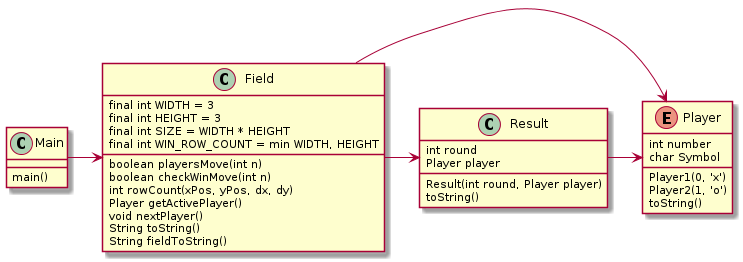
\includegraphics[scale=0.45]{3A}
\end{frame}


\begin{frame}[fragile]{Übungsblatt 3A - Objektorientierte Programmierung}
 \begin{multicols}{2}
 \lstinputlisting[basicstyle=\scriptsize]{3A.iuml}
 \end{multicols}

\end{frame}

%best solution
\begin{frame}[fragile]{Übungsblatt 3A - Objektorientierte Programmierung}
 \begin{multicols}{2}
 \lstinputlisting[basicstyle=\tiny]{solution/Field.java}
 \end{multicols}

\end{frame}

\begin{frame}[fragile]{Übungsblatt 3A - Objektorientierte Programmierung}
 \lstinputlisting[basicstyle=\scriptsize]{solution/Main.java}

\end{frame}

\begin{frame}[fragile]{Übungsblatt 3A - Objektorientierte Programmierung}
 \begin{multicols}{2}
 \lstinputlisting[basicstyle=\scriptsize]{solution/Player.java}
 \end{multicols}

\end{frame}

\begin{frame}[fragile]{Übungsblatt 3A - Objektorientierte Programmierung}
 \begin{multicols}{2}
 \lstinputlisting[basicstyle=\scriptsize]{solution/Result.java}
 \end{multicols}

\end{frame}

\section{Exceptions}

\subsection{Normale Exceptions}
\begin{frame}{Exceptions}

Exceptions werden verwendet um
\begin{itemize}
 \item Ausnahmefälle anzuzeigen
 \item Fehlerbehandlung durchzuführen
\end{itemize}

Exceptions sollten nicht verwendet werden um
\begin{itemize}
 \item den Programmablauf zu ändern
\end{itemize}
 
\end{frame}


\begin{frame}[fragile]{Beispiele}
\begin{figure}
   \begin{lstlisting}
    public class Test {
	  private static int test = 5;
	  public static void ifException (){
		  try {
			  if (test == 5) {
				  throw new Exception();
			  }
			  test = 7;

		  } catch (Exception e){
			  test = 5;
		  }
	  }
	  public static void main(String[] args){
		  ifException();
		  System.out.println(test);
	  }
    }
  \end{lstlisting}
\end{figure}

\only<2>{\vspace{-20em}\hspace{8em}
\includegraphics[scale=0.7]{X}}

\end{frame}

\begin{frame}[fragile]{Beispiele}
\begin{figure}
   \begin{lstlisting}
    public class Test {
	  private static int test = 5;
	  public static void ifException (){
		  try {
			  while (true) {
				  if (test == 500)
				    throw new Exception();
				  test++;
			  }
		  } catch (Exception e){
		    System.out.println("Schön dich hier zu sehen");			  
		  }
	  }
	  public static void main(String[] args){
		  ifException();
		  System.out.println(test);
	  }
    }
  \end{lstlisting}
\end{figure}

\only<2>{\vspace{-20em}\hspace{8em}
\includegraphics[scale=0.7]{X}}

\end{frame}


\begin{frame}[fragile]{Beispiele}
\begin{figure}
   \begin{lstlisting}
    public class Test {
	 public static void main(String[] args){
	    String test = "5";
	    int out = 3;
	    try {
	      out = Integer.parseInt(test);
	    } catch NumberFormatException e {
	      System.out.println("Error, using standard value 3");
	    }
	    System.out.println(out);
	 }
    }
  \end{lstlisting}
\end{figure}
\vfill
\only<2>{\vspace{-5em}\hspace{20em}
\includegraphics[scale=0.7]{Y}}

\end{frame}

\subsection{Runtime-Exceptions}
\begin{frame}[fragile]{Runtime Exceptions}
 Müssen nicht gecatched oder mittels throws ausgewiesen werden.
 Eigene Exceptions mittels \verb|extend RuntimeException|
 
 Wichtige RuntimeExceptions
 \begin{itemize}
  \item IllegalArgumentException
  \item IllegalStateException
  \item IndexOutOfBoundsException
  \item NullPointerException
 \end{itemize}

\end{frame}

\begin{frame}[fragile]{Beispiel - Runtime Exception}
 \begin{lstlisting}
  public class Test {
    public static double sqrt(double x) {
      if (x < 0) {
        throw new IllegalArgumentException();
      }
    }
  }
 \end{lstlisting}

\end{frame}


\begin{frame}[fragile]{Throws}
\begin{exampleblock}{BadFormatException.java}
 

\begin{lstlisting}
 public class BadFormatException extends Exception {
   public BadFormatException() {}
   public BadFormatException(String s){ super(s) }
 }
\end{lstlisting}
\end{exampleblock}
\begin{exampleblock}{Test.java}
 \begin{lstlisting}
  public class Test {
    public static void readFile (String path)  throws BadFormatException {
      if (x < 0) {
        throw new IllegalArgumentException();
      }
    }
  }
 \end{lstlisting}
\end{exampleblock}
\end{frame}



\begin{frame}[fragile]{Throws}
\begin{exampleblock}{BadFormatException.java}
 

\begin{lstlisting}
 public class BadFormatException extends RuntimeException {
   public BadFormatException() {}
   public BadFormatException(String s){ super(s) }
 }
\end{lstlisting}
\end{exampleblock}
\begin{exampleblock}{Test.java}
 \begin{lstlisting}
  public class Test {
    public static void readFile (String path) {
      if (x < 0) {
        throw new IllegalArgumentException();
      }
    }
  }
 \end{lstlisting}
\end{exampleblock}
\end{frame}

\begin{frame}[fragile]{Testing}
\begin{exampleblock}{UtilityClass.java}
 \begin{lstlisting}
  
public class UtilityClass {
  /**
   * @return The nth. fibonacci number
   * 
   */
  public int fib(int n) {
	  if (n == 0) return 0;
	  if (n == 1) return 1;
	  return fib(n-1) + fib(n-2);
	  
  }
}
 \end{lstlisting}
 \end{exampleblock}
for more see \url{http://www.vogella.com/tutorials/JUnit/article.html}
\end{frame}

\begin{frame}{Frohe Weihnachten}
 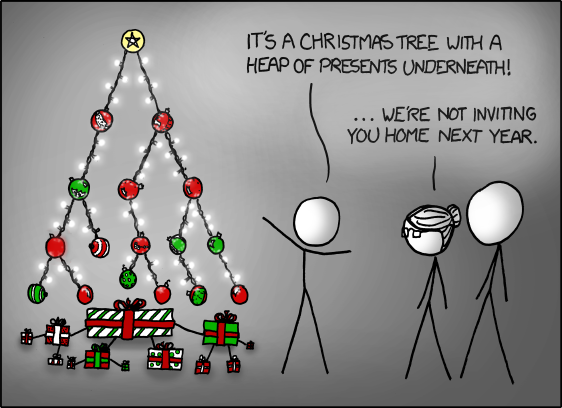
\includegraphics[scale=0.5]{08_tree}
 Quelle: http://xkcd.com/835
\end{frame}
\end{document}
